\documentclass{article}%
\usepackage[T1]{fontenc}%
\usepackage[utf8]{inputenc}%
\usepackage{lmodern}%
\usepackage{textcomp}%
\usepackage{lastpage}%
\usepackage[head=40pt,margin=0.5in,bottom=0.6in]{geometry}%
\usepackage{graphicx}%
%
\title{\textbf{Gobierno expulsó al embajador de Alemania}}%
\author{YAZMÍN ANTÍA}%
\date{07/03/2019}%
%
\begin{document}%
\normalsize%
\maketitle%
\textbf{URL: }%
http://www.eluniversal.com/politica/34964/gobierno{-}expulso{-}al{-}embajador{-}de{-}alemania\newline%
%
\textbf{Periodico: }%
EU, %
ID: %
34964, %
Seccion: %
politica\newline%
%
\textbf{Palabras Claves: }%
NO\_TIENE\newline%
%
\textbf{Derecho: }%
2.1%
, Otros Derechos: %
\newline%
%
\textbf{\textit{Canciller alemán consideró "incomprensible" la medida}}%
\newline%
\newline%
%
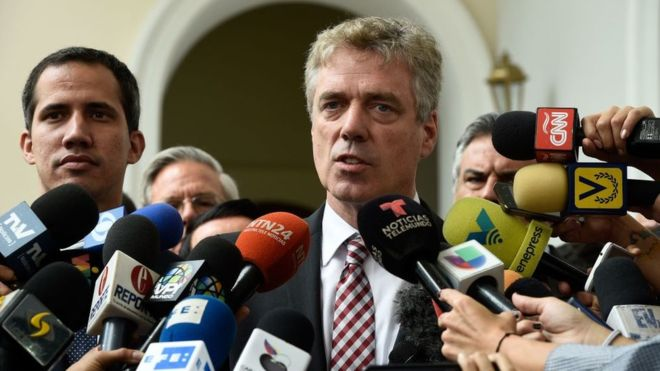
\includegraphics[width=300px]{EU_34964.jpg}%
\newline%
%
El gobierno de Nicolás Maduro declaró este miércoles persona "non grata" al embajador de Alemania, Martín Kriener, por supuestas actividades injerencistas y le otorgó 48 horas para abandonar el país.%
\newline%
%
En el Twitter del ministro de Relaciones Exteriores, Jorge Arreaza, se lee el comunicado de la Cancillería, donde afirman que la decisión obedece a los "recurrentes actos de injerencia en los asuntos internos del país" por parte del diplomático, tras presentarse, el pasado lunes, a recibir en el Aeropuerto de Maiquetía a Juan Guaidó, reconocido como presidente interino por más de 50 países, entre ellos, Alemania.%
\newline%
%
En el terminal aéreo cercano a Caracas, a la llegada de Guaidó, Kreiner estaba acompañado de representantes diplomáticos de varios países, incluso suramericanos, pero por el momento se tomó esta decisión sólo contra el embajador alemán, destaca la nota de la agencia AFP.%
\newline%
%
El Ministerio de Relaciones Exteriores señaló  que es "inaceptable que un representante diplomático extranjero ejerza en su territorio un rol público más propio de un dirigente político en clara alineación a la agenda" de la oposición venezolana.%
\newline%
%
Igualmente indican que no aceptaran intromisiones de extranjeros en "asuntos de competencia exclusiva" de venezolanos.%
\newline%
%
En respuesta, el ministro de Exteriores alemán, Heiko Maas, decidió llamar "a consultas" a su embajador en Venezuela, Daniel Kriener.~"Es una decisión incomprensible que agrava la situación y no contribuye a la distensión", expresa un breve comunicado del ministro compartido por las redes sociales.%
\newline%
%
En la nota diplomática, el ministro alemán de Asuntos Exteriores apuntó que "nuestro apoyo, el apoyo de Europa, a Juan Guaidó se mantiene intacto. El embajador Kreiner ha hecho un excelente trabajo en Caracas, en particular en los últimos días", afirmó.%
\newline%
%
Una amenaza%
\newline%
%
Por su parte, el jefe legislativo, Juan Guaidó, expresó que la decisión oficial contra el diplomático Kriener, debe ser tomada "como una amenaza".%
\newline%
%
Posteó que "el Embajador de la República de Alemania en Venezuela, Daniel Kriener, cuenta con nuestro total respaldo y reconocimiento". Habló de su absoluto compromiso con nuestra democracia, su respeto a nuestra constitución y su solidaridad.%
\newline%
%
"venezuela no es una amenaza"%
\newline%
%
La cancillería de la República expresó este miércoles el rechazo del Gobierno nacional a la anunciada extensión por parte del presidente estadounidense, Donald Trump, de la orden ejecutiva suscrita por el jefe del Ejecutivo de EEUU, Barack Obama, en marzo de 2015, en la que se declaraba a Venezuela como "amenaza inusual y extraordinaria para la seguridad nacional y la política exterior de Estados Unidos". A través de un comunicado, califican como paradójico que después de amenazar  al pueblo venezolano con una intervención militar, afirmando continuamente que "todas las opciones están sobre la mesa", el gobierno de EEUU pretenda hacer creer que se siente amenazado por Venezuela.%
\newline%
%
Se indica en dicho documento que "para la inmensa mayoría de los países del mundo resulta inconcebible que la primera potencia militar del planeta, que no desaprovecha la menor oportunidad para violar el derecho internacional y que hace uso de la fuerza en beneficio de sus propios intereses, pretenda calificar a Venezuela de "amenaza".%
\newline%
%
\end{document}